\documentclass[aspectratio=169]{beamer}
\usetheme{Copenhagen}
%% Remove draft for real article, put twocolumn for two columns
\usetheme{metropolis}
\usepackage{multicol}
\usepackage[style=british]{csquotes}

\def\signed #1{{\leavevmode\unskip\nobreak\hfil\penalty50\hskip1em
  \hbox{}\nobreak\hfill #1%
  \parfillskip=0pt \finalhyphendemerits=0 \endgraf}}

\newsavebox\mybox
\newenvironment{aquote}[1]
  {\savebox\mybox{#1}\begin{quote}\openautoquote\hspace*{-.7ex}}
  {\unskip\closeautoquote\vspace*{1mm}\signed{\usebox\mybox}\end{quote}}

\usepackage[utf8]{inputenc}
\newtheorem*{question}{Question}

\newcommand{\vectorproj}[2][]{\mathrm{proj}_{\vect{#1}}\vect{#2}}
\newcommand{\vectorcomp}[2][]{\mathrm{comp}_{\vect{#1}}\vect{#2}}
\newcommand{\vect}{\mathbf}
\newcommand{\R}{\mathbb{R}}
%% commentary bubble
\newcommand{\SV}[2][]{\sidenote[colback=green!10]{\textbf{SV\xspace #1:} #2}}

\title{ Multivariable Calculus \\ Day  15\\ Optimization (cont.) }
\date{Spring 2023}

\begin{document}

\maketitle

\begin{frame}
    \frametitle{Constrained optimization}
Constrained optimization takes various forms, depending on the assumptions.
We will deal with the most straight forward form.
The problem we will study is the following:

Maximize/minimize a function \(f:D\to \mathbb{R}\), subject to a constraint (side condition)
of the form
\(g(\mathbf{x}) = k\), for some constant \(k\in \mathbb{R}\).


Typically, people will write as follows
\begin{equation*}
\begin{aligned}
& \underset{x}{\text{minimize}}
& & f(x) \\
& \text{subject to}
& & 
g(x) = k \,.
\end{aligned}
\end{equation*}
\end{frame}

\begin{frame}
    \frametitle{Constrained optimization}
    
\begin{theorem}[Method of Lagrange Multiplier]

Suppose the maximum/minimum values of \(f\) exist and \(\nabla g(\mathbf{x}) \not=0\) where \(g(\mathbf{x}) = k\).
To find the maximum and minimum values of \(f\) subject to constraint
\(g(\mathbf{x}) = k\), we do the following:

\begin{enumerate}
\def\labelenumi{\arabic{enumi}.}
\item
  Find all values of \(\mathbf{x}\) and \(\lambda \in \mathbb{R}\) such that
  \begin{equation*}
   \nabla f(\mathbf{x}) =\lambda \nabla g(\mathbf{x})\,,
  \end{equation*}
  and
  \begin{equation*}
   g(\mathbf{x}) = k \,.
  \end{equation*}
\item
  Evaluate \(f\) at all the points \(\mathbf{x}\) that result from step 1. The largest of
  these values is the maximum of \(f\); the smallest is the minimum value of \(f\).
\end{enumerate}

\end{theorem}
\end{frame}

\begin{frame}
    \frametitle{Example}
    \url{https://youtu.be/hQ4UNu1P2kw}
\end{frame}

\begin{frame}
    \frametitle{Worksheet}
         Find the points on the sphere $x^2 + y^2 + z^2 =4$
            that are closest to and farthest from the point 
            $(1,1,1)$.
\end{frame}

\begin{frame}
    \frametitle{Two constraints}
        Problem 15 from \url{https://activecalculus.org/multi/S-10-8-Lagrange-Multipliers.html}

        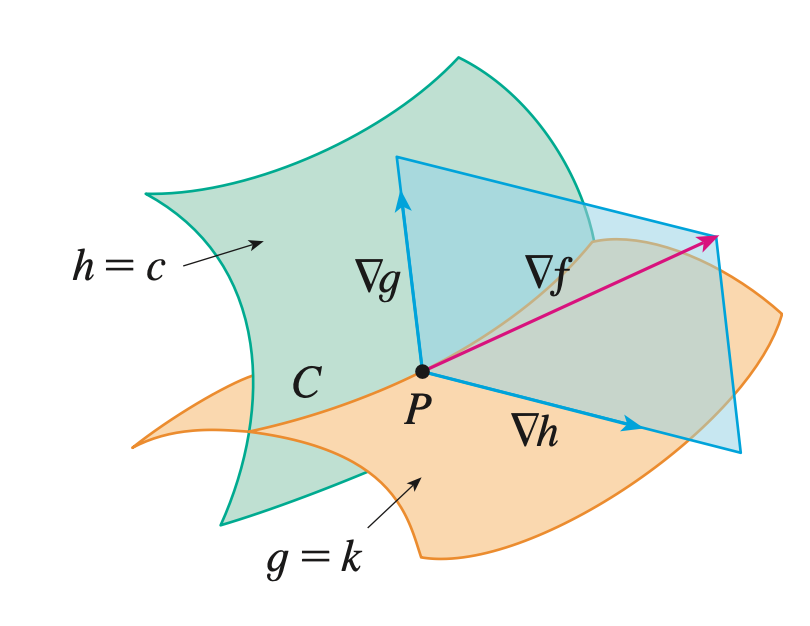
\includegraphics[scale=0.5]{two-constraints.png}
\end{frame}

\end{document}

